\documentclass[t]{beamer}
\usetheme[deutsch]{KIT}
\setbeamercovered{transparent}
\setbeamertemplate{navigation symbols}{}

\KITfoot{Tutoriumsmaterial von Alexander Kwiatkowski, Michael Vollmer und Matthias Holoch \hspace{2.5cm} Basierend auf den Folien von Simon Stroh und Moritz v. Looz}
\usepackage[utf8]{inputenc}
\usepackage{amsmath}
\usepackage{ifthen}
\usepackage{amssymb}
\usepackage{tikz}
\usepackage{ngerman}
\usepackage[normalem]{ulem}
\usetikzlibrary{automata}
\usenavigationsymbols


\title{Theoretische Grundlagen der Informatik}
\subtitle{Tutorium}
\author{Alexander Kwiatkowski, Michael Vollmer und Matthias Holoch}

\institute[IKS]{Institut für Kryptographie und Sicherheit}

\TitleImage[height=\titleimageht]{images/tmaschine.png}

\newcommand{\N}{\ensuremath{\mathbb{N}}}
\newcommand{\M}{\ensuremath{\mathcal{M}}}
\newcommand{\classP}{\ensuremath{\mathcal{P}}}
\newcommand{\classNP}{\ensuremath{\mathcal{NP}}}
\newcommand{\co}{\ensuremath{\mathsf{co\text{-}}}}
\newcommand{\pot}{\ensuremath{\mathcal{P}}}
\newcommand{\abs}[1]{\ensuremath{\left\vert #1 \right\vert}}
\newcommand{\menge}[2]{\ensuremath{\left\lbrace #1 \,\middle\vert\, #2 \right\rbrace}}
\newcommand{\ducttape}[1]{\vspace{#1}}
\newcommand{\neglit}[1]{\overline{#1\vphantom{x^a}}}
\newcommand{\recipe}{\raisebox{-.3cm}{
\includegraphics[scale=.15]{images/chefs-cap.png}}\hspace{0.2cm}}
\newcommand{\opt}[1]{\ensuremath{\text{OPT}(#1)}}
\newcommand{\A}[1]{\ensuremath{\mathcal{A}(#1)}}
\renewcommand{\O}[1]{\ensuremath{\mathcal{O}(#1)}}
\newcommand{\msout}[1]{\text{\sout{\ensuremath{#1}}}}

\newcommand{\invincible}{\setbeamercovered{invisible}} %  "Yesss! I am invincible!!" (Boris Grishenko)
\newcommand{\vincible}{\setbeamercovered{transparent}}
\renewcommand{\solution}[1]{\invincible \pause #1 \vincible}
\newcommand{\micropause}{\\[8pt]}

% \@ifundefined{tikzset}{}{\tikzset{initial text=}} % Text "start" bei Startknoten unterdrücken
\tikzstyle{every node}=[thick]
\tikzstyle{every line}=[thick]

\newcommand{\tutnr}[1]{
  \subtitle{Tutorium #1}
	\begin{frame}
		\maketitle
	\end{frame}
}

\newcommand{\uebnr}[1]{
  \subtitle{Anmerkungen zum #1. Übungsblatt}
	\begin{frame}
		\maketitle
	\end{frame}
}

\begin{document}

\newcommand{\start}[3]
{
  \draw (#1*2,#2*2) node{$#3$};
  \draw (#1*2,#2*2) circle(0.4cm);
  \draw [->] (#1*2-0.9,#2) -- (#1*2-0.4,#2);
}
\newcommand{\final}[3]
{
  \draw (#1*2,#2*2) node{$#3$};
  \draw (#1*2,#2*2) circle(0.4cm);
  \draw (#1*2,#2*2) circle(0.32cm);
}
\newcommand{\startfinal}[3]
{
  \draw (#1*2,#2*2) node{$#3$};
  \draw (#1*2,#2*2) circle(0.4cm);
  \draw (#1*2,#2*2) circle(0.32cm);
  \draw [->] (#1*2-0.9,#2) -- (#1*2-0.4,#2);
}
\newcommand{\state}[3]
{
  \draw (#1*2,#2*2) node{$#3$};
  \draw (#1*2,#2*2) circle(0.4cm);
}
\newcommand{\tol}[4]
{
  \draw (#1+#3,#2*2) node[above]{$#4$};
  \draw [->] (#1*2-0.4,#2*2) -- (#3*2+0.4,#2*2);
}
\newcommand{\tor}[4]
{
  \draw (#1+#3,#2*2) node[above]{$#4$};
  \draw [->] (#1*2+0.4,#2*2) -- (#3*2-0.4,#2*2);
}
\newcommand{\tot}[4]
{
  \draw (#1*2,#2+#3) node[right]{$#4$};
  \draw [->] (#1*2,#2*2+0.4) -- (#1*2,#3*2-0.4);
}
\newcommand{\tob}[4]
{
  \draw (#1*2,#2+#3) node[right]{$#4$};
  \draw [->] (#1*2,#2*2-0.4) -- (#1*2,#3*2+0.4);
}
\newcommand{\totl}[5]
{
  \draw (#1+#3,#2+#4) node[above right]{$#5$};
  \draw [->] (#1*2-0.283,#2*2+0.283) -- (#3*2+0.283,#4*2-0.283);
}
\newcommand{\totr}[5]
{
  \draw (#1+#3,#2+#4) node[above left]{$#5$};
  \draw [->] (#1*2+0.283,#2*2+0.283) -- (#3*2-0.283,#4*2-0.283);
}
\newcommand{\tobl}[5]
{
  \draw (#1+#3,#2+#4) node[below right]{$#5$};
  \draw [->] (#1*2-0.283,#2*2-0.283) -- (#3*2+0.283,#4*2+0.283);
}
\newcommand{\tobr}[5]
{
  \draw (#1+#3,#2+#4) node[below left]{$#5$};
  \draw [->] (#1*2+0.283,#2*2-0.283) -- (#3*2-0.283,#4*2+0.283);
}
\newcommand{\rloopl}[3]
{
  \draw (#1*2-1,#2*2) node[left]{$#3$};
  \draw [->] (#1*2-0.35,#2*2-0.2) arc (-30:-320:0.32cm);
}
\newcommand{\rloopr}[3]
{
  \draw (#1*2+1,#2*2) node[right]{$#3$};
  \draw [->] (#1*2+0.35,#2*2+0.2) arc (150:-140:0.32cm);
}
\newcommand{\rloopt}[3]
{
  \draw (#1*2,#2*2+1) node[above]{$#3$};
  \draw [->] (#1*2-0.2,#2*2+0.35) arc (240:-50:0.32cm);
}
\newcommand{\rloopb}[3]
{
  \draw (#1*2,#2*2-1) node[below]{$#3$};
  \draw [->] (#1*2+0.2,#2*2-0.35) arc (60:-230:0.32cm);
}
\newcommand{\lloopl}[3]
{
  \draw (#1*2-1,#2*2) node[left]{$#3$};
  \draw [->] (#1*2-0.35,#2*2+0.2) arc (30:320:0.32cm);
}
\newcommand{\lloopr}[3]
{
  \draw (#1*2+1,#2*2) node[right]{$#3$};
  \draw [->] (#1*2+0.35,#2*2-0.2) arc (-150:140:0.32cm);
}
\newcommand{\lloopt}[3]
{
  \draw (#1*2,#2*2+1) node[above]{$#3$};
  \draw [->] (#1*2+0.2,#2*2+0.35) arc (-60:230:0.32cm);
}
\newcommand{\lloopb}[3]
{
  \draw (#1*2,#2*2-1) node[below]{$#3$};
  \draw [->] (#1*2-0.2,#2*2-0.35) arc (-240:50:0.32cm);
}
\include{amsmath}

\tutnr{10}

\section{Informationsquellen}
\subsection{Informationsquellen}
\begin{frame}
\frametitle{look-up}
\begin{itemize}
	\item Vorlesungsfolien
	\begin{itemize}
		\item http://www.iks.kit.edu/index.php?id=tgi-ws12
	\end{itemize}
	\item Tutoriumsfolien
	\begin{itemize}
		\item tinyurl.com/tgi1213
		\item Neue Position des Download-Ordners~\\
		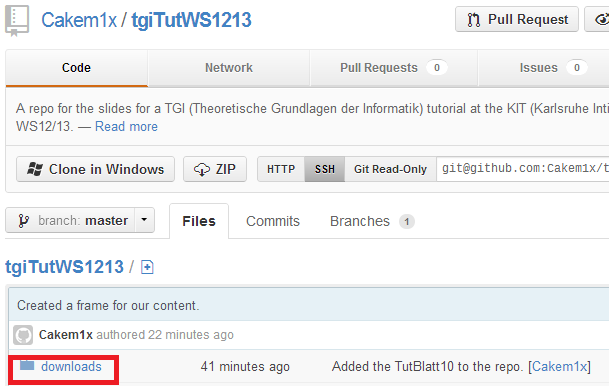
\includegraphics[scale=0.2]{images/download.png}
	\end{itemize}
	\item Michael Sipser, Introduction to the Theory of Computation
	\begin{itemize}
		\item Grundlage der Vorlesung
		\item Eher zum Nachschlagen empfohlen
	\end{itemize}
	\item Vorlesungs-Skript
	\begin{itemize}
		\item In Arbeit
		\item Unter Umständen sehr geringe Zeitspanne zwischen Veröffentlichung des Skripts und der Klausur
	\end{itemize}
\end{itemize}
\end{frame}

\section{Aufgaben zu P, NP}
\subsection{Aufgabe B10 A2}
\begin{frame}
	\frametitle{Aufgabe B10 A2}
	Finden Sie den Fehler im folgenden ``Beweis'' f"ur \textbf{P} $\not=$ \textbf{NP}!\\
	Betrachten Sie folgenden Algorithmus f"ur SAT:\\[4pt]
	- Durchlaufe f"ur die gegebene Formel $\phi$ alle m"oglichen Belegungen der
	Variablen mit den Wahrheitswerten\\
	- Akzeptiere $\phi$, wenn eine der durchlaufenen Belegungen $\phi$ erf"ullt\\[4pt]
	Dieser Algorithmus hat eine mit der Anzahl der Variablen exponentiell wachsende
	Laufzeit. Daher hat das Problem SAT einen exponentiellen Aufwand und kann nicht in
	\textbf{P} liegen. Weil aber SAT in \textbf{NP} liegt, mu"s also \textbf{P} $\not=$
	\textbf{NP} gelten.
\end{frame}
\subsection{Aufgabe B10 A3}
\begin{frame}
	\frametitle{Aufgabe B10 A3}
	\begin{enumerate}
		\item Zeigen Sie, dass es unter der Voraussetzung \textbf{P} $=$ \textbf{NP} m"oglich
		ist, f"ur eine aussagenlogische Formel $\phi$ in\\
		polynomieller Zeit eine erf"ullende Belegung der Variablen zu finden, falls eine
		solche Belegung existiert!
	\end{enumerate}
\end{frame}

\section{HALF-CLIQUE}
\subsection{HALF-CLIQUE}
\subsection{Aufgabe B10 A1}
\begin{frame}
	\frametitle{Aufgabe B10 A1}
	Gegeben ist das folgende Problem:
	\begin{tabbing}
	HALF-CLIQUE:\\
	\textit{Gegeben:} \= Ein ungerichteter Graph $G = (V,E)$\\
	\textit{Gesucht:} \> Gibt es eine Teilmenge $V' \subseteq V$\\
	\> mit	$\forall \; v,w \in V', v \not= w: (v,w) \in E$ und $|V'| \geq |V|/2$
	\end{tabbing}
	Beweisen Sie, dass HALF-CLIQUE \textbf{NP}-vollst"andig ist!\\[4pt]
	\underline{Zur Erinnerung:}\\
	Das als \textbf{NP}-vollst"andig bekannte Problem CLIQUE ist definiert durch:
	\begin{tabbing}
	CLIQUE:\\
	\textit{Gegeben:} \= Ein ungerichteter Graph $G = (V,E)$ und $k \in \mathbb{N}$\\
	\textit{Gesucht:} \> Gibt es eine Teilmenge $V' \subseteq V$\\
	\> mit	$\forall \; v,w \in V', v \not= w: (v,w) \in E$ und $|V'| \geq k$
	\end{tabbing}
\end{frame}

\section{Hamiltonkreis und TSP}
\subsection{Hamiltonkreis}
\begin{frame}
	\frametitle{Hamiltonkreis}
	\begin{block}{Kurzdefinition}
	Enthält der gegebene Graph einen Kreis, d.h. gibt es einen Pfad der durch jeden Knoten exakt einmal geht und vom Startknoten wieder zum Startknoten führt (Start- und Endknoten wird nur einmal gezählt).
	\end{block}
	\begin{block}{Formal}
	Gegeben: Ein ungerichteter Graph $G=(V,E)$.\\
	Gesucht: Besitzt $G$ einen Hamiltonkreis? (Dies ist eine Permutation $\pi$ der Knotenindizes ($v_{\pi(1)}$, $v_{\pi(2)}$,...,$v_{\pi(n)}$), sodass für $i=1,...,n-1$ gilt: $\{v_{\pi(i)},v_{\pi(i+1)}\}\in E$) und 
außerdem $\{v_{\pi(n)},v_{\pi(1)}\} \in E)$.
	\end{block}
\end{frame}
\begin{frame}
	\frametitle{Beispiel}
	Gibt es in diesem Graphen einen Hamiltonkreis?
	\begin{center}
		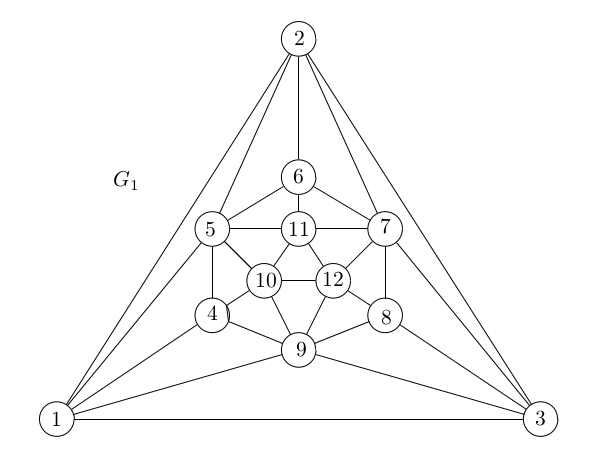
\includegraphics[scale=0.4]{images/4_Faerben}
	\end{center}
\end{frame}
\subsection{Travelling Salesman}
\begin{frame}
	\frametitle{Travelling Salesman}
	\begin{block}{Kurzdefinition}
	Geben sie einen Kreis des gegeben vollständig verbundenen Graphen mit Kantenlängen an, sodass dessen Gesamtkantenlänge minimal ist.
	\end{block}
	\begin{block}{Formal}
	Gegeben: Ein Graph $G=(V,V \times V)$\\
	Gesucht: Ein einfacher Kreis $C=(v_1,v_2,...,v_n,v_1)$, sodass $n=|V|$ und $\sum_{(u,v)\in C} d(u,v)$ minimiert wird, wobei $d(u,v)$ die Entfernung zwischen den Knoten $u$ und $v$ ist.\\
	\end{block}
\end{frame}
\begin{frame}
	\frametitle{Beispiel}
	Wie lang ist die kürzeste Route und durch welche Kanten geht sie?
	\begin{center}		
		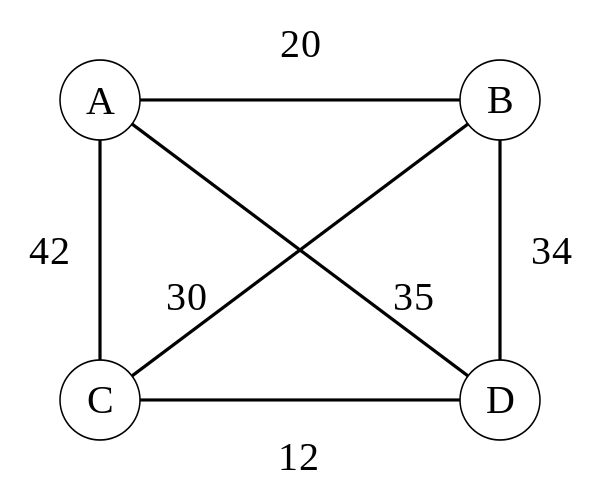
\includegraphics[scale=0.5]{images/Weighted_K4}
	\end{center}
\end{frame}
\subsection{Aufgabe B10 A4}
\begin{frame}
	\frametitle{Aufgabe B10 A4}
 Gegeben sind folgende Probleme: 
 \begin{tabbing}
 \textbf{Hamiltonkreisproblem:} \\
 \hspace{10pt} \= \textit{Gegeben:} \= Ein ungerichteter Baum $G=(V,E)$.\\
 \> \textit{Gesucht:} \> Besitzt $G$ einen Hamiltonkreis? (Dies ist eine Permutation $\pi$\\
 \> der Knotenindizes ($v_{\pi(1)}$,$v_{\pi(2)}$,...,$v_{\pi(n)}$), sodass für $i=1,...,n-1$ gilt:\\
 \> $\{v_{\pi(i)},v_{\pi(i+1)}\}\in E$) und außerdem $\{v_{\pi(n)},v_{\pi(1)}\} \in E)$.\\ \\
 \textbf{Travelling Salesman(TSP):}\\
 \> \textit{Gegeben:} Ein Graph $G=(V,V \times V)$\\
 \> \textit{Gesucht:} \> Ein einfacher Kreis $C=(v_1,v_2,...,v_n,v_1)$, sodass $n=|V|$\\ 
 \> und $\sum_{(u,v)\in C} d(u,v)$ minimiert wird, wobei $d(u,v)$ die Entfernung\\ 
 \>zwischen den Knoten $u$ und $v$ ist.\\
\end{tabbing}
Zeigen Sie, dass TSP NP-Vollständig ist, wobei das Hamiltonkreisproblem auch NP-Vollständig ist. Benutzen Sie für den Beweis die Reduktion Hamiltonkreisproblem$\leq_p$TSP. 
\end{frame}
\begin{frame}
	\frametitle{Aufgabe B10 A4}
Gegeben sei folgender Graph:\newline
\begin{center}
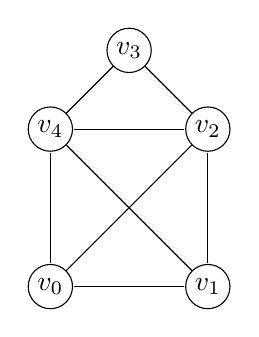
\begin{tikzpicture}
 \draw (0,0) circle (8pt);
 \draw (0,0) node {$v_0$};
 \draw (2,0) circle (8pt);
 \draw (2,0) node {$v_1$};
 \draw (2,2) circle (8pt);
 \draw (2,2) node {$v_2$};
 \draw (1,3) circle (8pt);
 \draw (1,3) node {$v_3$};
 \draw (0,2) circle (8pt);
 \draw (0,2) node {$v_4$};
 \draw (0.2,0.2) -- (1.8,1.8);
 \draw (0.2,1.8) -- (1.8,0.2);
 \draw (0.2,2.2) -- (0.8,2.8);
 \draw (1.2,2.8) -- (1.8,2.2);
 \draw (0.3,0) -- (1.7,0);
 \draw (0.3,2) -- (1.7,2);
 \draw (0,0.3) -- (0,1.7);
 \draw (2,0.3) -- (2,1.7);
\end{tikzpicture}
\end{center}
Gibt es einen Hamiltonkreis? Wandeln Sie hierzu das Problem in ein TSP um und finden Sie eine optimale Rundtour.
\end{frame}

\section{Schluss}
\subsection{Schluss}
\begin{frame}
\frametitle{Bis zum nächsten Mal!}
\begin{center}
	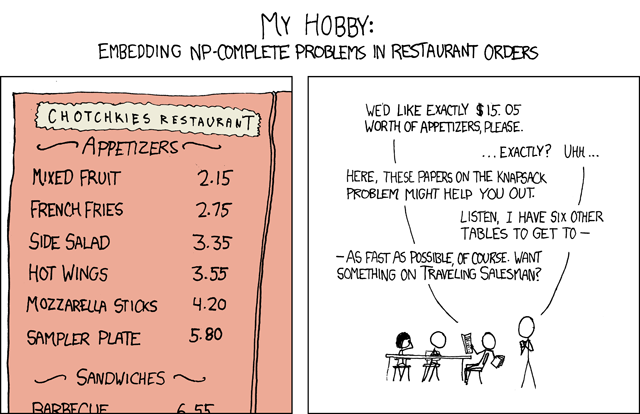
\includegraphics[scale=5.2]{images/287_np_complete.png}
\end{center}
\end{frame}

\frame{
  \frametitle{Lizenzen}
  \center
  
\includegraphics[width=2em]{images/by}
  
\includegraphics[width=2em]{images/cc}
  
\includegraphics[width=2em]{images/sa}
  \\
  {\tiny

Dieses Werk ist unter einem ``Creative Commons Namensnennung-Weitergabe unter gleichen Bedingungen 3.0 Deutschland``-Lizenzvertrag lizenziert. Um eine Kopie der Lizenz zu erhalten, gehen Sie bitte zu \href{http://creativecommons.org/licenses/by-sa/3.0/de/}{http://creativecommons.org/licenses/by-sa/3.0/de/} oder schreiben Sie an Creative Commons, 171 Second Street, Suite 300, San Francisco, California 94105, USA.\\
  \vspace{1cm}
  Davon ausgenommen sind das Titelbild, welches aus der März-April 2002 Ausgabe von American Scientist erschienen ist und ohne Erlaubnis verwendet wird, sowie das KIT Beamer Theme. Hierfür gelten die Bestimmungen der jeweiligen Urheber.
  \vspace{1cm}
  \\ 
  }
  %Habe hier die Reihenfolge etwas umgestellt, weil die Formatierung bei mir komisch aussah. 
  %Wenn es bei dir anders ist, kannst du es auch wieder zurückändern, dann haben wir unterschiedliche Kompilieroptionen
}

\end{document}